\chapter{Cromatografia}\label{ch:b2:chromatography}

Uma gota de bebida energética, diluída e filtrada, é injetada em um tubo de aço não mais longo que uma
caneta e recheado de grãos de sílica de alguns micrômetros. Alguns minutos depois, um detector traçou uma
linha com um punhado de picos, e a partir da área de um deles o laboratório informa quanta cafeína a
lata contém, com precisão de alguns por cento. A \omterm{def:b2:chromatography:principle}{cromatografia} separa os componentes de uma mistura
fazendo-os correr através de uma coluna a velocidades diferentes; este capítulo explica por que eles
viajam a velocidades diferentes, por que seus picos têm a largura que têm, como separar dois vizinhos, e
como transformar um pico em uma quantidade.

\begin{omfigure}
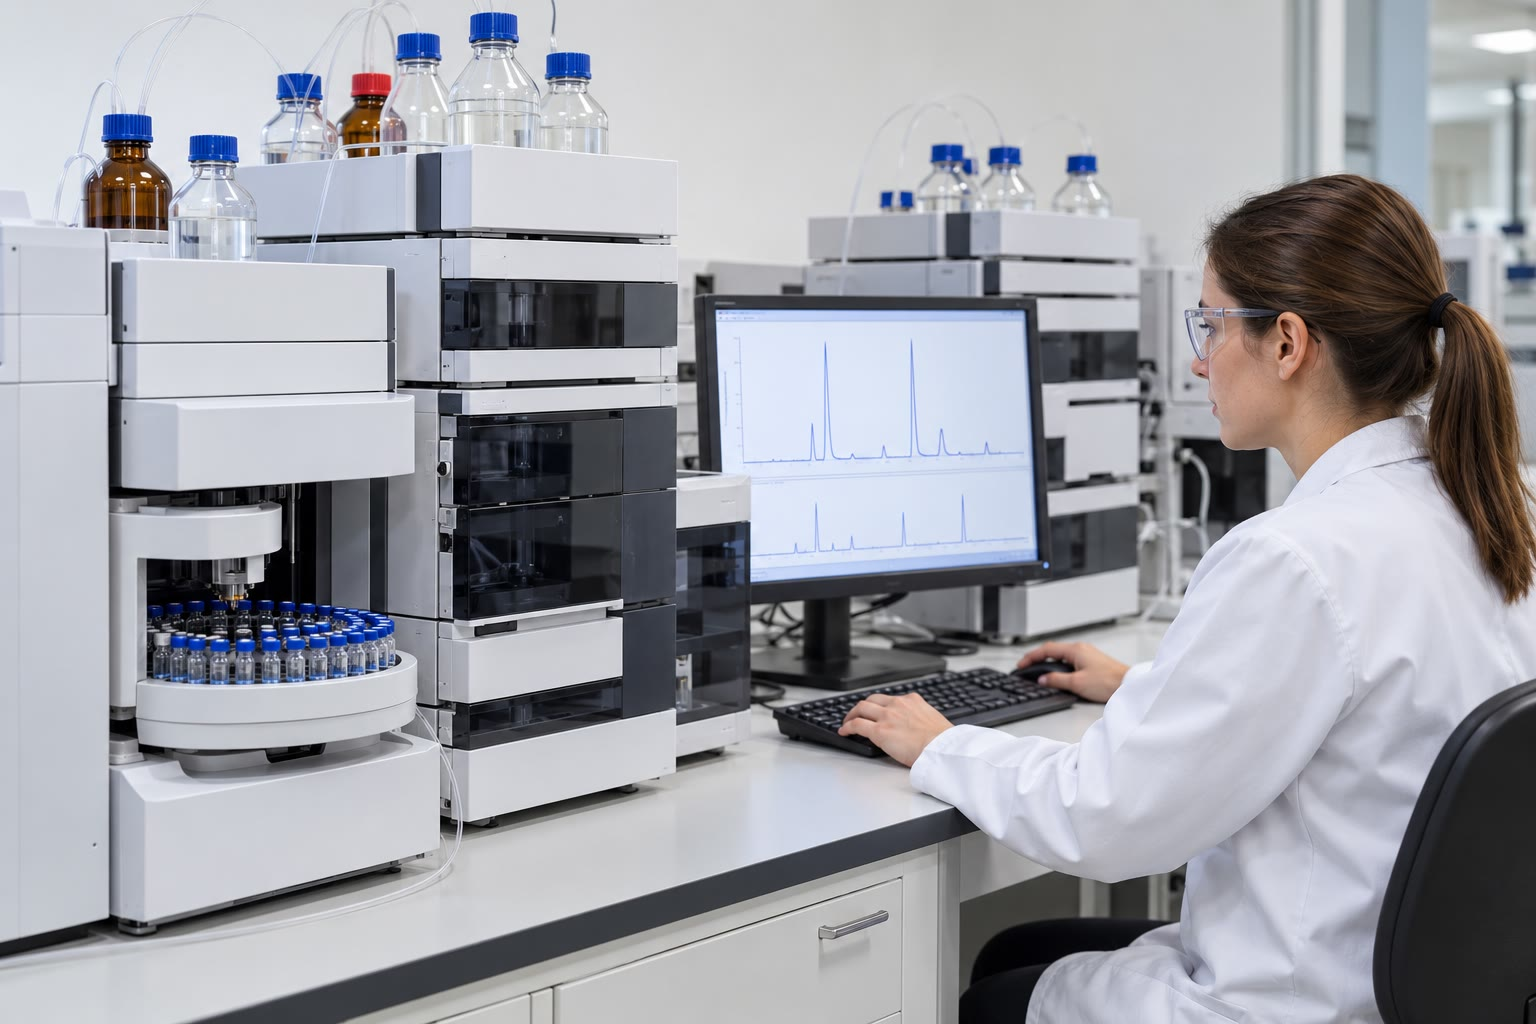
\includegraphics[width=0.58\linewidth]{images/book3/ai/b2-31-analytical-lab.jpg}

{\small Um laboratório de análises: cromatógrafos a líquido com seus frascos de solvente e uma bandeja
de amostrador automático cheia de frascos; os cromatogramas aparecem na tela (ilustração).}
\end{omfigure}

\begin{recall}
O volume escolar: \omterm{def:b2:chromatography:principle}{cromatografia} em papel e em camada delgada, cromatograma, eluente. O volume do 1.º
ano: o coeficiente de partição, a extração líquido--líquido, o fator de retenção $R_f$ de uma placa de
camada delgada. \Cref{ch:b2:liquid-vapour-diagrams}: o \omterm{def:b2:liquid-vapour-diagrams:fractional-distillation}{prato teórico} de uma coluna de destilação.
\end{recall}

\section{Princípio}

\begin{definition}[Cromatografia]\label{def:b2:chromatography:principle}
A \emph{cromatografia}\index{cromatografia} separa os componentes de uma mistura distribuindo-os entre
uma \emph{fase estacionária}\index{fase estacionaria@fase estacionária}, fixada em uma coluna ou em uma placa, e uma
\emph{fase móvel}\index{fase movel@fase móvel}, um gás ou um líquido que escoa ao longo dela. Arrastar os componentes
através da coluna e para fora dela com a fase móvel é a \emph{eluição}\index{eluicao@eluição}.
\end{definition}

Uma molécula só avança enquanto está na \omterm{def:b2:chromatography:principle}{fase móvel}; enquanto está retida pela \omterm{def:b2:chromatography:principle}{fase estacionária}, ela
espera. Ela passa de uma fase à outra milhões de vezes em seu trajeto, de modo que sua velocidade média
é fixada pela fração do tempo que passa em cada uma, isto é, por seu equilíbrio de partição.

\begin{definition}[Retenção]\label{def:b2:chromatography:retention}
O \emph{tempo de retenção}\index{tempo de retencao@tempo de retenção} $t_R$ de um composto é o tempo entre a injeção e o
máximo de seu pico; o \emph{tempo morto}\index{tempo morto} $t_M$ é o tempo de retenção de um composto
não retido, que nunca entra na \omterm{def:b2:chromatography:principle}{fase estacionária}. O \emph{fator de retenção}\index{fator de retencao k@fator de retenção $k$}
$k$ de um composto em uma coluna é
\begin{equation*}
k = \frac{t_R - t_M}{t_M}.
\end{equation*}
Ele não é o $R_f$ de uma placa de camada delgada, que mede uma distância percorrida, embora ambos
descrevam a mesma partição.
\end{definition}

\begin{proposition}[Tempo de retenção]\label{prop:b2:chromatography:retention-time}
Se, no equilíbrio, as quantidades de um composto nas \omterm{def:b2:chromatography:principle}{fases estacionária} e móvel de uma fatia de coluna
são $n_s$ e $n_m$, o composto avança a $u/(1 + n_s/n_m)$, onde $u$ é a velocidade da \omterm{def:b2:chromatography:principle}{fase móvel},
e $t_R = t_M(1 + n_s/n_m)$.
\end{proposition}

\begin{proof}
Uma molécula dada passa a fração $n_m/(n_s + n_m)$ de seu tempo na \omterm{def:b2:chromatography:principle}{fase móvel}, onde avança a
$u$, e o resto parada. Sua velocidade média é $u\,n_m/(n_s + n_m) = u/(1 + n_s/n_m)$. A coluna de
comprimento $L$ é atravessada em $t_R = (L/u)(1 + n_s/n_m)$, e $L/u = t_M$.
\end{proof}

\begin{proposition}[Retenção e partição]\label{prop:b2:chromatography:k-and-K}
O \omterm{def:b2:chromatography:retention}{fator de retenção} é a razão das quantidades nas duas fases, $k = n_s/n_m = KV_s/V_m$, onde $K$
é o coeficiente de partição (concentração na \omterm{def:b2:chromatography:principle}{fase estacionária} sobre concentração na \omterm{def:b2:chromatography:principle}{fase
móvel}) e $V_s$, $V_m$ os volumes das fases na coluna.
\end{proposition}

\begin{proof}
Pela \cref{prop:b2:chromatography:retention-time}, $(t_R - t_M)/t_M = n_s/n_m$. Com $n_s = c_sV_s$,
$n_m = c_mV_m$ e $K = c_s/c_m$, $n_s/n_m = KV_s/V_m$.
\end{proof}

Dois compostos se separam se seus coeficientes de partição diferem; a geometria da coluna ($V_s/V_m$)
multiplica todas as retenções igualmente. Mudar a \omterm{def:b2:chromatography:principle}{fase móvel}, o que muda $K$, é a principal alavanca
do químico sobre a retenção.

\begin{omfigure}
\begin{tikzpicture}[x=1cm, y=1cm]
\foreach \x/\a/\b/\ha/\hb/\lab in {0/0.6/0.6/0.1/0.1/início, 2.4/1.5/2.6/0.16/0.22/depois, 4.8/2.4/4.4/0.2/0.3/fim}{
  \draw[black!60] (\x-0.35,0) rectangle (\x+0.35,-5);
  \fill[omThm!55] (\x-0.33,-\b+\hb) rectangle (\x+0.33,-\b-\hb);
  \fill[omDef!55, opacity=0.85] (\x-0.33,-\a+\ha) rectangle (\x+0.33,-\a-\ha);
  \node[font=\small] at (\x,-5.4) {\lab};
}
\draw[->, thick] (-1.0,-0.3) -- (-1.0,-4.6) node[midway, left, font=\small, align=right] {fase\\móvel};
\node[font=\small, align=left, anchor=west] at (5.5,-2.4) {mais retido\\(lento, estreito)};
\node[font=\small, align=left, anchor=west] at (5.5,-4.4) {menos retido\\(rápido)};
\draw[densely dotted] (5.15,-2.4) -- (5.5,-2.4); \draw[densely dotted] (5.15,-4.4) -- (5.5,-4.4);
\end{tikzpicture}
\par\vspace{4pt}

{\small Dois compostos injetados juntos como uma única banda fina descem por uma coluna (três
instantâneos, esquema). O menos retido ($k$ menor) corre à frente; as duas bandas se alargam ao viajar,
tanto mais quanto mais longe foram.}
\end{omfigure}

\section{Largura de pico e número de pratos}

Uma banda não permanece fina. As moléculas de um mesmo composto seguem caminhos diferentes entre os
grãos, difundem ao longo da coluna e se atrasam na \omterm{def:b2:chromatography:principle}{fase estacionária} em quantidades aleatórias. O pico
registrado na saída é quase exatamente uma gaussiana de desvio-padrão $\sigma_t$ (em tempo), e quanto
mais estreito ele é para um dado $t_R$, melhor a coluna.

\begin{definition}[Número de pratos]\label{def:b2:chromatography:plates}
O \emph{número de pratos}\index{numero de pratos@número de pratos} de uma coluna para um composto é $N = (t_R/\sigma_t)^2$, onde
$\sigma_t$ é o desvio-padrão de seu pico em tempo. A \emph{altura de prato}\index{altura de prato} é
$H = L/N$, para uma coluna de comprimento $L$.
\end{definition}

Os nomes vêm da coluna de destilação do \cref{ch:b2:liquid-vapour-diagrams}: uma coluna
cromatográfica se comporta como se fosse uma pilha de $N$ estágios de equilíbrio, cada um de altura $H$.
A analogia é uma maneira de contar, não uma imagem da coluna.

\begin{proposition}[Número de pratos a partir de um pico]\label{prop:b2:chromatography:plate-number}
Com $w$ a largura na base entre as tangentes nos pontos de inflexão e $w_{1/2}$ a largura a
meia altura,
\begin{equation*}
N = 16\left(\frac{t_R}{w}\right)^2 = 5.54\left(\frac{t_R}{w_{1/2}}\right)^2.
\end{equation*}
\end{proposition}

\begin{proof}
Para uma gaussiana de desvio-padrão $\sigma$ e altura $h$, os pontos de inflexão estão em $\pm\sigma$,
onde a altura é $h\mathrm e^{-1/2}$ e a inclinação $\mp h\mathrm e^{-1/2}/\sigma$; a tangente ali
atinge zero após mais $\sigma$, em $\pm2\sigma$: $w = 4\sigma$. A meia altura é atingida onde
$\mathrm e^{-x^2/2\sigma^2} = 1/2$, $x = \sigma\sqrt{2\ln2}$: $w_{1/2} = 2\sqrt{2\ln2}\,\sigma \approx
2.355\,\sigma$. Substituir $\sigma = w/4$ ou $\sigma = w_{1/2}/2.355$ em $N = (t_R/\sigma)^2$ dá
$16$ e $2.355^2 = 5.545$, escrito 5.54.
\end{proof}

\begin{proposition}[Equação de van Deemter]\label{prop:b2:chromatography:van-deemter}
A \omterm{def:b2:chromatography:plates}{altura de prato} depende da velocidade linear $u$ da \omterm{def:b2:chromatography:principle}{fase móvel} segundo
\begin{equation*}
H = A + \frac{B}{u} + Cu,
\end{equation*}
onde $A$ representa os diferentes caminhos através do recheio, $B/u$ a difusão ao longo da coluna
(pior quando as moléculas ficam mais tempo) e $Cu$ a troca lenta com a \omterm{def:b2:chromatography:principle}{fase estacionária} (pior
quando a \omterm{def:b2:chromatography:principle}{fase móvel} passa depressa). $H$ é mínima em $u_{\mathrm{opt}} = \sqrt{B/C}$, onde $H_{\min} =
A + 2\sqrt{BC}$.
\end{proposition}

\admitted

A forma da equação é admitida; seu mínimo, não. $\mathrm dH/\mathrm du = -B/u^2 + C$ se anula
em $u = \sqrt{B/C}$, e ali $B/u = Cu = \sqrt{BC}$, logo $H_{\min} = A + 2\sqrt{BC}$; a derivada
segunda $2B/u^3$ é positiva, portanto trata-se de um mínimo. Grãos pequenos reduzem $A$ e $C$: é por
isso que a \omterm{def:b2:chromatography:principle}{cromatografia} líquida moderna usa partículas de alguns micrômetros e altas pressões para
empurrar a \omterm{def:b2:chromatography:principle}{fase móvel} através delas.

\begin{omfigure}
\begin{tikzpicture}
\begin{axis}[width=0.7\linewidth, height=5.2cm, xmin=0, xmax=8, ymin=0, ymax=70,
  xlabel={velocidade linear $u$ (\unit{mm/s})}, ylabel={altura de prato $H$ (\unit{\micro m})},
  label style={font=\small}, tick label style={font=\scriptsize},
  legend style={font=\scriptsize, at={(1.03,1)}, anchor=north west}, legend cell align=left]
\addplot[omDef, very thick] table[x=u, y=H] {figdata/out/bachelor-2-chromatogram-b.dat};
\addplot[black!50, dashed] table[x=u, y=A] {figdata/out/bachelor-2-chromatogram-b.dat};
\addplot[omThm, dashed] table[x=u, y=B] {figdata/out/bachelor-2-chromatogram-b.dat};
\addplot[omMeth, dashed] table[x=u, y=C] {figdata/out/bachelor-2-chromatogram-b.dat};
\addplot[only marks, mark=*, mark size=1.6pt] coordinates {(2,30)};
\legend{$H$, $A$, $B/u$, $Cu$}
\end{axis}
\end{tikzpicture}

{\small Uma curva de van Deemter (parâmetros do exercício: $A = \qty{10}{\micro m}$, $B = \qty{20}{\micro m.mm/s}$,
$C = \qty{5}{\micro m.s/mm}$). O mínimo, $H = \qty{30}{\micro m}$ em $u = \qty{2}{mm/s}$, fica onde
os termos de difusão e de troca são iguais.}
% figdata: bachelor-2/chromatogram.py part b
\end{omfigure}

\section{Separar dois compostos}

\begin{definition}[Seletividade e resolução]\label{def:b2:chromatography:separation}
Para dois picos vizinhos com $k_2 > k_1$, o \emph{fator de seletividade}\index{fator de seletividade} é
$\alpha = k_2/k_1$, e a \emph{resolução}\index{resolucao@resolução} é
\begin{equation*}
R_s = \frac{2(t_{R2} - t_{R1})}{w_1 + w_2},
\end{equation*}
a distância entre os picos dividida por sua largura média na base.
\end{definition}

Com $R_s = 1$ os picos ainda se sobrepõem visivelmente; com $R_s = 1.5$ o sinal volta à linha de base
entre eles (separação até a linha de base), que é o objetivo habitual em trabalho quantitativo.

\begin{omfigure}
\begin{tikzpicture}
\begin{axis}[width=0.36\linewidth, height=3.6cm, xmin=-8, xmax=8, ymin=0, ymax=1.15,
  xtick=\empty, ytick=\empty, axis x line=bottom, axis y line=none, title style={font=\small},
  title={$R_s = 0.75$}]
\addplot[omDef, thick] table[x=x, y=r075] {figdata/out/bachelor-2-chromatogram-a.dat};
\end{axis}
\end{tikzpicture}\hfill\begin{tikzpicture}
\begin{axis}[width=0.36\linewidth, height=3.6cm, xmin=-8, xmax=8, ymin=0, ymax=1.15,
  xtick=\empty, ytick=\empty, axis x line=bottom, axis y line=none, title style={font=\small},
  title={$R_s = 1.0$}]
\addplot[omDef, thick] table[x=x, y=r100] {figdata/out/bachelor-2-chromatogram-a.dat};
\end{axis}
\end{tikzpicture}\hfill\begin{tikzpicture}
\begin{axis}[width=0.36\linewidth, height=3.6cm, xmin=-8, xmax=8, ymin=0, ymax=1.15,
  xtick=\empty, ytick=\empty, axis x line=bottom, axis y line=none, title style={font=\small},
  title={$R_s = 1.5$}]
\addplot[omDef, thick] table[x=x, y=r150] {figdata/out/bachelor-2-chromatogram-a.dat};
\end{axis}
\end{tikzpicture}

{\small Dois picos gaussianos de mesmo tamanho a três \omterm{def:b2:chromatography:separation}{resoluções} (modelo). A 0.75 eles se fundem em
um dubleto; a 1.0 o vale ainda está a um quarto da altura; a 1.5 o sinal está de volta à linha de
base.}
% figdata: bachelor-2/chromatogram.py part a
\end{omfigure}

\begin{theorem}[Equação da resolução]\label{thm:b2:chromatography:resolution}
Para dois picos vizinhos com o mesmo \omterm{def:b2:chromatography:plates}{número de pratos} $N$,
\begin{equation*}
R_s = \frac{\sqrt N}{4}\,\frac{\alpha - 1}{\alpha}\,\frac{k_2}{1 + k_2}.
\end{equation*}
\end{theorem}

\begin{proof}
Para picos próximos, as duas larguras na base são quase iguais; tomemos ambas iguais à do segundo pico,
$w = 4\sigma_t = 4t_{R2}/\sqrt N$ (\cref{def:b2:chromatography:plates}). Então $R_s = (t_{R2} -
t_{R1})/w = \sqrt N\,(t_{R2} - t_{R1})/(4t_{R2})$. Com $t_R = t_M(1 + k)$
(\cref{prop:b2:chromatography:retention-time}), $t_{R2} - t_{R1} = t_M(k_2 - k_1)$ e $t_{R2} =
t_M(1 + k_2)$, logo $R_s = (\sqrt N/4)(k_2 - k_1)/(1 + k_2)$. Por fim, $k_2 - k_1 = k_2(1 - 1/\alpha) =
k_2(\alpha - 1)/\alpha$.
\end{proof}

\begin{method}[Melhorar uma resolução]\label{met:b2:chromatography:improve-resolution}
\begin{enumerate}
  \item Eficiência: $R_s \propto \sqrt N$. Dobrar o comprimento da coluna dobra $N$ e o tempo de
        análise, mas multiplica $R_s$ por apenas $\sqrt2 \approx 1.41$; partículas menores ou a vazão
        ótima aumentam $N$ a comprimento constante.
  \item Seletividade: o fator $(\alpha - 1)/\alpha$ é o mais sensível. Mude a \omterm{def:b2:chromatography:principle}{fase móvel}
        (solvente, pH), a \omterm{def:b2:chromatography:principle}{fase estacionária} ou, em \omterm{def:b2:chromatography:techniques}{cromatografia gasosa}, a temperatura.
  \item Retenção: $k_2/(1+k_2)$ sobe rapidamente até $k \approx 2$ e lentamente além disso, enquanto o
        tempo continua a crescer como $1 + k$; vise $k$ entre cerca de 2 e 10.
\end{enumerate}
\end{method}

\section{As técnicas}

\begin{definition}[Técnicas cromatográficas]\label{def:b2:chromatography:techniques}
Na \emph{cromatografia gasosa}\index{cromatografia gasosa} (CG), a \omterm{def:b2:chromatography:principle}{fase móvel} é um gás (hélio, hidrogênio ou
nitrogênio) e a \omterm{def:b2:chromatography:principle}{fase estacionária} um filme líquido que reveste o interior de uma longa coluna capilar,
mantida em um forno. Na \emph{cromatografia líquida de alta eficiência}\index{cromatografia liquida de alta eficiencia@cromatografia líquida de alta eficiência}
(CLAE), uma bomba empurra uma \omterm{def:b2:chromatography:principle}{fase móvel} líquida através de uma coluna curta recheada de pequenas
partículas. Na CLAE em \emph{fase reversa}\index{fase reversa}, a \omterm{def:b2:chromatography:principle}{fase estacionária} é apolar
(sílica que leva longas cadeias alquila) e a \omterm{def:b2:chromatography:principle}{fase móvel} uma mistura polar de água com metanol ou
acetonitrila. Na \emph{eluição por gradiente}\index{eluicao por gradiente@eluição por gradiente}, a composição da \omterm{def:b2:chromatography:principle}{fase móvel} é
modificada durante a corrida, em \omterm{def:b2:chromatography:principle}{cromatografia} líquida, para eluir mais depressa os compostos
fortemente retidos.
\end{definition}

\begin{omfigure}
\begin{tikzpicture}[x=1cm, y=1cm, box/.style={draw=black!70, rounded corners=2pt, fill=white,
  font=\small, align=center, minimum height=0.8cm, inner sep=3pt}]
\node[box] (gas) at (0,0) {gás de\\arraste};
\node[box] (inj) at (2.2,0) {injetor\\aquecido};
\draw[black!70, rounded corners=2pt, fill=omDef!8] (3.5,-1.1) rectangle (6.5,1.1);
\node[font=\small] at (5,0.85) {forno};
\draw[omDef, thick] (5,-0.15) circle (0.55); \draw[omDef, thick] (5,-0.15) circle (0.42);
\node[box] (det) at (8.0,0) {detector};
\node[box] (data) at (10.2,0) {sistema de\\dados};
\draw[->, thick] (gas) -- (inj);
\draw[->, thick] (inj.east) -- (4.45,0);
\draw[->, thick] (5.55,0) -- (det.west);
\draw[->, thick] (det) -- (data);
\node[font=\footnotesize, align=center] at (5,-1.45) {coluna capilar (enrolada)};
\end{tikzpicture}

\medskip
\begin{tikzpicture}[x=1cm, y=1cm, box/.style={draw=black!70, rounded corners=2pt, fill=white,
  font=\small, align=center, minimum height=0.8cm, inner sep=3pt}]
\node[box] (sol) at (0,0) {reservatórios\\de solvente};
\node[box] (pump) at (2.4,0) {bomba de\\alta pressão};
\node[box] (inj) at (4.9,0) {injetor};
\draw[black!70, fill=omThm!12] (6.2,-0.18) rectangle (8.2,0.18);
\node[font=\footnotesize] at (7.2,0.45) {coluna recheada};
\node[box] (uv) at (9.6,0) {célula\\UV};
\node[box] (data) at (11.5,0) {dados};
\draw[->, thick] (sol) -- (pump); \draw[->, thick] (pump) -- (inj);
\draw[->, thick] (inj) -- (6.2,0); \draw[->, thick] (8.2,0) -- (uv); \draw[->, thick] (uv) -- (data);
\end{tikzpicture}
\par\vspace{4pt}

{\small Diagramas de blocos. Em cima: um cromatógrafo a gás; a amostra é vaporizada no injetor, levada
pelo gás através de uma coluna capilar de dezenas de metros enrolada em um forno, e detectada na saída.
Embaixo: um cromatógrafo a líquido; a bomba mistura os solventes (\omterm{def:b2:chromatography:techniques}{eluição por gradiente}) e os empurra a
alta pressão através de uma coluna recheada curta até uma célula de absorbância UV.}
\end{omfigure}

A escolha entre elas decorre da volatilidade. A CG exige compostos que se vaporizem sem se decompor,
aproximadamente abaixo de \qty{400}{\degreeCelsius}: solventes, combustíveis, fragrâncias, pequenas
moléculas orgânicas. Elevar a temperatura do forno durante a corrida (uma rampa de temperatura) elui
mais cedo os compostos mais pesados, como faz um gradiente em CLAE. A CLAE trata tudo o que se
dissolve, incluindo sais, açúcares, fármacos e proteínas. Em \omterm{def:b2:chromatography:techniques}{fase reversa}, os compostos mais polares
saem primeiro e os mais apolares por último; acrescentar mais solvente orgânico à \omterm{def:b2:chromatography:principle}{fase móvel} diminui
todas as retenções. A \omterm{def:b2:chromatography:principle}{cromatografia} em coluna preparativa, e sua versão mais rápida, a \omterm{def:b2:chromatography:principle}{cromatografia}
\textit{flash}, aplicam o mesmo princípio em grande escala para purificar gramas de produto, em geral
sobre sílica polar com misturas de hexano e acetato de etila.

\section{Análise quantitativa}

A área de um pico é proporcional à quantidade de composto que chegou ao detector, mas a constante de
proporcionalidade depende do composto e do detector. Os volumes injetados, da ordem do microlitro, não
são perfeitamente reprodutíveis. Um \omterm{def:b2:chromatography:quantitative}{padrão interno} elimina as duas dificuldades.

\begin{definition}[Fator de resposta e padrão interno]\label{def:b2:chromatography:quantitative}
Um \emph{padrão interno}\index{padrao interno@padrão interno} é um composto, ausente da amostra, acrescentado em
quantidade conhecida a toda solução analisada; ele deve ser resolvido de todos os outros picos e se
comportar como o analito. O \emph{fator de resposta}\index{fator de resposta} $F$ de um analito em relação
ao padrão interno é definido por
\begin{equation*}
\frac{A_X}{A_{IS}} = F\,\frac{c_X}{c_{IS}},
\end{equation*}
onde $A$ são áreas de pico e $c$ concentrações na solução injetada.
\end{definition}

\begin{proposition}[Quantificação por padrão interno]\label{prop:b2:chromatography:internal-standard}
$F$ medido em uma solução de calibração de $c_X$ e $c_{IS}$ conhecidos dá, para uma amostra dopada com o
\omterm{def:b2:chromatography:quantitative}{padrão interno} a $c_{IS}$, $c_X = (A_X/A_{IS})\,c_{IS}/F$, qualquer que seja o volume injetado.
\end{proposition}

\begin{proof}
Cada área é proporcional à quantidade injetada: $A_X = s_X c_X v$, $A_{IS} = s_{IS} c_{IS} v$, com
as sensibilidades do detector $s$ e o volume injetado $v$. A razão $A_X/A_{IS} = (s_X/s_{IS})(c_X/c_{IS})$
já não contém $v$, e $F = s_X/s_{IS}$ é uma constante do método, medida uma vez na solução de
calibração. Isolar $c_X$ dá o resultado.
\end{proof}

\begin{method}[Quantificar com um padrão interno]\label{met:b2:chromatography:internal-standard}
\begin{enumerate}
  \item Escolha um padrão de estrutura próxima à do analito, ausente da amostra, eluindo perto dele mas
        resolvido ($R_s \ge 1.5$).
  \item Injete uma solução de calibração de $c_X$ e $c_{IS}$ conhecidos; calcule $F$ a partir da razão das áreas.
  \item Acrescente o padrão à solução da amostra na mesma $c_{IS}$; injete; leia $A_X/A_{IS}$.
  \item Calcule $c_X = (A_X/A_{IS})\,c_{IS}/F$, e depois remonte todas as diluições até a amostra
        original.
\end{enumerate}
\end{method}

Uma calibração externa (uma série de padrões do analito sozinho, depois a amostra, todos injetados da
mesma maneira) é mais simples, mas supõe que o volume injetado e o detector permaneçam constantes
entre as corridas.

\begin{history}[A escrita das cores, 1906]
\begin{minipage}[t]{0.18\linewidth}
\vspace{0pt}
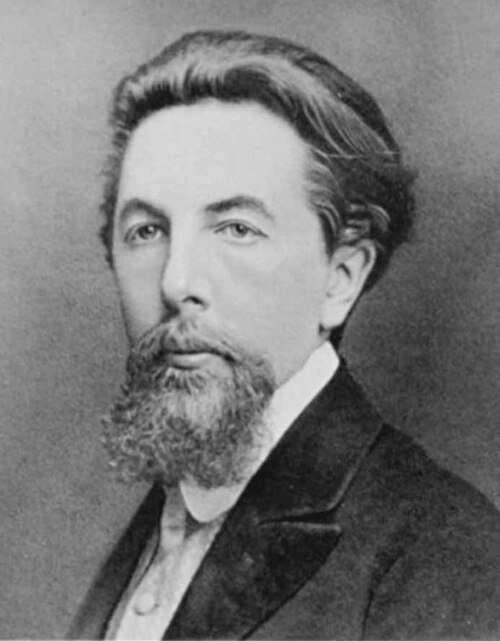
\includegraphics[width=\linewidth]{images/book3/tsvet.jpg}
\end{minipage}\hfill
\begin{minipage}[t]{0.78\linewidth}
\vspace{0pt}
O botânico Mikhail Tsvet derramou um extrato de folhas verdes em um tubo de vidro cheio de giz em pó e
o lavou com um solvente: os pigmentos se separaram em bandas coloridas, clorofilas verdes e
carotenoides amarelos. Em 1906 ele chamou o método de \omterm{def:b2:chromatography:principle}{cromatografia}, ``escrita das cores''. Ele foi
amplamente ignorado durante um quarto de século, até ser retomado para os produtos naturais nos anos
1930. (Retrato: autor desconhecido, domínio público; Wikimedia Commons.)
\end{minipage}
\end{history}

\begin{safety}{\ghs[5mm]{GHS02}\,\ghs[5mm]{GHS05}\,\ghs[5mm]{GHS06}\,\ghs[5mm]{GHS07}\,\ghs[5mm]{GHS08}\,\ghs[5mm]{GHS09}}
A acetonitrila e o metanol, os componentes orgânicos habituais das \omterm{def:b2:chromatography:principle}{fases móveis} de CLAE, são inflamáveis
e tóxicos; o hexano, usado em \omterm{def:b2:chromatography:principle}{cromatografia} em coluna, é inflamável, perigoso para a saúde e tóxico para
a vida aquática. Os resíduos de solvente são recolhidos, nunca despejados na pia.
% ledger: ghs:acetonitrile, ghs:methanol, ghs:hexane
\end{safety}

\section{Exercícios}

\begin{exercise}[$\star$]\label{exo:b2:chromatography:1}
Um composto tem $t_R = \qty{5.0}{min}$ em uma coluna cujo \omterm{def:b2:chromatography:retention}{tempo morto} é \qty{1.0}{min}. Calcule seu
\omterm{def:b2:chromatography:retention}{fator de retenção} e a fração de seu tempo passada na \omterm{def:b2:chromatography:principle}{fase móvel}.
\end{exercise}

\begin{exercise}[$\star$]\label{exo:b2:chromatography:2}
Um pico em $t_R = \qty{6.0}{min}$ tem uma largura na base de \qty{0.30}{min}. Calcule o \omterm{def:b2:chromatography:plates}{número de pratos}.
\end{exercise}

\begin{exercise}[$\star$]\label{exo:b2:chromatography:3}
Uma coluna de \qty{250}{mm} dá $N = 10\,000$ para um composto. Calcule a \omterm{def:b2:chromatography:plates}{altura de prato}.
\end{exercise}

\begin{exercise}[$\star$]\label{exo:b2:chromatography:4}
CG ou CLAE? Etanol no sangue; uma proteína; cafeína em uma bebida; benzeno na gasolina; açúcares em um suco de fruta.
\end{exercise}

\begin{exercise}[$\star\star$]\label{exo:b2:chromatography:5}
Dois picos: $t_{R1} = \qty{4.0}{min}$, $w_1 = \qty{0.40}{min}$; $t_{R2} = \qty{4.6}{min}$, $w_2 =
\qty{0.50}{min}$. Calcule a \omterm{def:b2:chromatography:separation}{resolução}. Eles estão separados até a linha de base?
\end{exercise}

\begin{exercise}[$\star\star$]\label{exo:b2:chromatography:6}
Quantos pratos são necessários para separar dois compostos com $\alpha = 1.10$ e $k_2 = 4.0$ com
$R_s = 1.5$?
\end{exercise}

\begin{exercise}[$\star\star$]\label{exo:b2:chromatography:7}
Uma coluna tem $A = \qty{5}{\micro m}$, $B = \qty{8}{\micro m.mm/s}$, $C = \qty{2}{\micro m.s/mm}$
(dados do exercício). Encontre a velocidade ótima e a menor \omterm{def:b2:chromatography:plates}{altura de prato}.
\end{exercise}

\begin{exercise}[$\star\star$]\label{exo:b2:chromatography:8}
Preveja a ordem de \omterm{def:b2:chromatography:principle}{eluição} do benzeno, do fenol e do tolueno em CLAE de \omterm{def:b2:chromatography:techniques}{fase reversa} com uma \omterm{def:b2:chromatography:principle}{fase móvel}
água--metanol, e o que acontece quando a fração de metanol é aumentada.
\end{exercise}

\begin{exercise}[$\star\star$]\label{exo:b2:chromatography:9}
Uma solução de calibração de um analito a \qty{20.0}{mg/L} com o \omterm{def:b2:chromatography:quantitative}{padrão interno} a \qty{10.0}{mg/L}
dá áreas 860 e 400. Uma amostra dopada com o padrão a \qty{10.0}{mg/L} dá áreas 645 e 410.
Calcule o \omterm{def:b2:chromatography:quantitative}{fator de resposta} e a concentração do analito (dados do exercício).
\end{exercise}

\begin{exercise}[$\star\star\star$]\label{exo:b2:chromatography:10}
Uma separação dá $R_s = 1.06$. Que comprimento de coluna, em relação ao atual, dá $R_s = 1.5$, e quanto
isso custa em tempo? Que outras alavancas existem?
\end{exercise}

\begin{exercise}[$\star\star\star$]\label{exo:b2:chromatography:11}
Para dois picos gaussianos de mesma altura e largura, com largura na base $w = 4\sigma$, calcule o sinal
a meio caminho entre eles, em relação à altura do pico, com $R_s = 1$ e com $R_s = 1.5$ (despreze a
contribuição do pico distante em cada máximo).
\end{exercise}

\begin{exercise}[$\star\star\star$]\label{exo:b2:chromatography:12}
Com $N$ e $\alpha$ constantes, compare o fator de \omterm{def:b2:chromatography:separation}{resolução} $k_2/(1+k_2)$ e o tempo relativo de análise
$1 + k_2$ para $k_2 = 2$, 5 e 10. Que faixa de $k$ você escolheria?
\end{exercise}

\section{Problema: A cafeína de uma bebida energética}

\begin{problem}[{Problema de fim de semana --- a ordem de eluição em fase reversa, o desempenho da
coluna a partir de um cromatograma, melhorar a separação, e a quantificação com um padrão interno}]
\label{pb:b2:chromatography:1}
Dados do exercício (inventados, não um método real). Uma bebida energética é diluída dez vezes (\qty{5.00}{mL}
em \qty{50.0}{mL}) e a teofilina é acrescentada como \omterm{def:b2:chromatography:quantitative}{padrão interno} a \qty{40.0}{mg/L} na solução
diluída. Coluna: \qty{150}{mm}, \omterm{def:b2:chromatography:techniques}{fase reversa}; \omterm{def:b2:chromatography:principle}{fase móvel} água--metanol; detecção UV. A
matriz não retida (açúcares e sais) elui em $t_M = \qty{1.0}{min}$; a teofilina em
\qty{3.0}{min} (largura na base \qty{0.18}{min}); a cafeína em \qty{3.4}{min} (largura na base \qty{0.20}{min}).
Calibração: cafeína \qty{50.0}{mg/L} e teofilina \qty{40.0}{mg/L} dão áreas 1500 e 1000.
Amostra: áreas 970 (cafeína) e 1010 (teofilina). Uma lata contém \qty{250}{mL}.
% ledger: ghs:caffeine, ghs:methanol

\begin{center}
\begin{tikzpicture}
\begin{axis}[width=0.75\linewidth, height=4.4cm, xmin=0, xmax=5, ymin=0, ymax=1,
  xlabel={tempo (min)}, ylabel={absorbância (u.a.)}, label style={font=\small},
  tick label style={font=\scriptsize}, ytick=\empty]
\addplot[omDef, thick] table[x=t, y=s] {figdata/out/bachelor-2-chromatogram-c.dat};
\node[font=\scriptsize] at (axis cs:1.0,0.42) {matriz};
\node[font=\scriptsize] at (axis cs:2.62,0.86) {teofilina};
\node[font=\scriptsize] at (axis cs:3.85,0.84) {cafeína};
\end{axis}
\end{tikzpicture}
\end{center}
% figdata: bachelor-2/chromatogram.py part c

\medskip
\noindent\textbf{Parte I --- \omterm{def:b2:chromatography:techniques}{Fase reversa}.}
\begin{enumerate}
  \item Descreva as \omterm{def:b2:chromatography:principle}{fases estacionária} e móvel de uma coluna de \omterm{def:b2:chromatography:techniques}{fase reversa}.
  \item Por que os açúcares eluem no \omterm{def:b2:chromatography:retention}{tempo morto}?
  \item A cafeína é a 1,3,7-trimetilxantina, a teofilina a 1,3-dimetilxantina. Explique sua ordem de
        \omterm{def:b2:chromatography:principle}{eluição}.
  \item Por que a teofilina é aqui um bom \omterm{def:b2:chromatography:quantitative}{padrão interno}?
  \item O que aconteceria com os dois \omterm{def:b2:chromatography:retention}{tempos de retenção} se a fração de metanol fosse aumentada?
  \item O que mede o \omterm{def:b2:chromatography:retention}{tempo morto}?
\end{enumerate}

\medskip
\noindent\textbf{Parte II --- Desempenho da coluna.}
\begin{enumerate}[resume]
  \item Calcule os \omterm{def:b2:chromatography:retention}{fatores de retenção} da teofilina e da cafeína.
  \item Calcule o \omterm{def:b2:chromatography:separation}{fator de seletividade}.
  \item Calcule o \omterm{def:b2:chromatography:plates}{número de pratos} para a cafeína e para a teofilina.
  \item Calcule a \omterm{def:b2:chromatography:plates}{altura de prato} para a cafeína.
  \item Calcule a \omterm{def:b2:chromatography:separation}{resolução} entre os dois picos.
  \item Verifique-a com a equação da \omterm{def:b2:chromatography:separation}{resolução}.
  \item Os picos estão separados até a linha de base?
\end{enumerate}

\medskip
\noindent\textbf{Parte III --- Mais rápido ou melhor.}
\begin{enumerate}[resume]
  \item Para ganhar tempo, a coluna é encurtada para \qty{75}{mm} (mesmo recheio e mesma vazão). O que
        acontece com a \omterm{def:b2:chromatography:separation}{resolução}?
  \item E com o tempo de análise?
  \item O que daria em vez disso uma coluna de \qty{300}{mm}, e a que custo?
  \item Que alavanca age sobre $\alpha$?
  \item Aumentar $k$ ajudaria muito aqui?
\end{enumerate}

\medskip
\noindent\textbf{Parte IV --- Quantificação.}
\begin{enumerate}[resume]
  \item Calcule o \omterm{def:b2:chromatography:quantitative}{fator de resposta} da cafeína em relação à teofilina.
  \item Por que o volume injetado não importa?
  \item Calcule a concentração de cafeína na solução diluída.
  \item Calcule a concentração de cafeína na bebida.
  \item O que daria errado se um composto da matriz coeluísse com a teofilina?
  \item O que uma calibração externa exigiria em vez disso?
  \item Dê a massa de cafeína em uma lata de \qty{250}{mL}.
\end{enumerate}
\end{problem}
